\documentclass[twoside,10pt]{article}
\usepackage{/Users/bradenhoagland/latex/styles/toggles}
%\toggletrue{sectionbreaks}
%\toggletrue{sectionheaders}
\newcommand{\docTitle}{HW 4}
\usepackage{/Users/bradenhoagland/latex/styles/common}
\importStyles{modern}{rainbow}{boxy}

%\renewcommand{\theenumi}{\alph{enumi}}

\begin{document}
%\tableofcontents

% ------------------------------
% Lesson 6, 5 points
% ------------------------------
\begin{exer}[Lesson 6, 5 points]
	If $f:K\to L$ is a simplicial map, show
	\begin{enumerate}
		\item $f_{\#}$ maps cycles to cycles.
		\item $f_{\#}$ maps boundaries to boundaries.
		\item The map
			\begin{align*}
				f_{*}:H_{\bullet}(K) &\to H_{\bullet}(L) \\
				[x] &\mapsto [f_{\#}(x)]
			\end{align*}
			is a well-defined linear map.
	\end{enumerate}
\end{exer}

\textbf{First two parts:} 
In class we proved that $f_{\#}$ respects the boundary operator in the sense that $f_{\#}\circ \p_{K} = \p_{L} \circ f_{\#}$, as proven in class. This implies that the following diagram commutes.
\[
	\begin{tikzcd}
		C_{p+1}^{K} \rar{\p_{K}} \dar{f_{\#}} & C_{p}^{K} \rar{\p_{K}} \dar{f_{\#}} & C_{p-1}^{L} \dar{f_{\#}} \\
		C_{p+1}^{L} \rar{\p_{L}} & C_{p}^{L} \rar{\p_{L}} & C_{p-1}^{L}
	\end{tikzcd}
\] We can show (1) and (2) through a diagram chase. Suppose $z \in Z_{p}^{K}$ is a cycle, then $(\p_{L}\circ f_{\#})(z) = (f_{\#} \circ \p_{K})(z) = f_{\#}(0) = 0$. Thus $f_{\#}(z)$ is also a cycle.

Now suppose $b \in B_{p}^{K}$, then there is some $a \in C_{p+1}^{K}$ such that $\p_{K}(a) = b$. Then $(\p_{L} \circ f_{\#})(a) = (f_{\#}\circ \p_{K})(a) = f_{\#}(b)$, i.e. $f_{\#}(b)$ is a boundary.

\textbf{Third part:} 
We now show that $f_{*}$ is a well-defined linear map. By (1), $f_{\#}(x)$ is a cycle if $x$ is a cycle; thus it makes sense to take the equivalence class $f_{*}(x) = [f_{\#}(x)]$. Also note that since $[x]=[y] \iff x-y \in \im  \p$, then (2) says that $f_{*}(x-y) = [f_{\#}(x-y)] = 0$. Then since $f_{\#}$ is linear,
\[
	f_{*}([x]) - f_{*}([y]) = [f_{\#}(x)] - [f_{\#}(y)] = [f_{\#}(x)-f_{\#}(y)] = [f_{\#}(x-y)] = 0.
\] Thus $f_{*}([x]) = f_{*}([y])$, so $f_{*}$ is well-defined. The linearity of $f_{\#}$ also implies
\[
	f_{*}(\mu[x]+\lambda[y]) = f_{*}([\mu x+\lambda y]) = [f_{\#}(\mu x + \lambda y)] = [\mu f_{\#}(x) + \lambda f_{\#}(y)] = \mu f_{*}([x]) + \lambda f_{*}([y]),
\] so $f_{*}$ is also linear.


\textbf{Alternative third part:} 
Consider the following diagram,
\[
\begin{tikzcd}
	Z_{p}^{K} \dar[two heads]{\pi_{K}} \rar{f_{\#}} & Z_{p}^{L} \dar[two heads]{\pi_{L}} \\
	H_{p}(K) \rar[dashed, "\exists!\;f_{*}"'] & H_{p}(L)
\end{tikzcd}
\] where $\pi$ is the canonical projection. The map $f_{\#}:Z_{p}^{K}\to Z_{p}^{L}$ is well-defined since $f_{\#}$ sends cycles to cycles. Since it also maps boundaries to boundaries, $B_{p}^{K} \subseteq \ker (\pi_{L}\circ f_{\#})$. Then by the universal property of quotients, there is a unique linear map $f_{*}$ making the diagram commute. By commutativity, this $f_{*}$ is exactly the $f_{*}$ defined in the problem.

\newpage

% ------------------------------
% Lesson 7, 5 points
% ------------------------------
\begin{exer}[Lesson 7, 5 points]
Compute $\beta_1$ and $\beta_2$ of the simplicial complex shown in the notes.
\end{exer}

The simplicial complex is pictured below. The four faces of the empty tetradhedron are in fact filled in, but the tetrahedron itself is not filled in.
\begin{figure}[H]
	\centering
	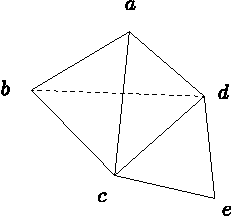
\includegraphics[scale=1]{fig/2.pdf}
	%\caption{}
\end{figure}

I wrote the attached code to put a matrix into Smith normal form. Since it uses only elementary row/column operations, rank is preserved, so $\text{rank}(\texttt{smith}(A)) = \text{rank}(A)$.

I start with the following matrices, where $A$ represents $\p_2$ and $B$ represents $\p_1$.
\begin{align*}
	A &=
	\begin{tabular}{c | c c c c}
		& abc & abd & acd & bcd \\
		\hline
		ab & 1 & 1 & 0 & 0 \\
		ac & 1 & 0 & 1 & 0 \\
		ad & 0 & 1 & 1 & 0 \\
		bc & 1 & 0 & 0 & 1 \\
		bd & 0 & 1 & 0 & 1 \\
		cd & 0 & 0 & 1 & 1 \\
		ce & 0 & 0 & 0 & 0 \\
		de & 0 & 0 & 0 & 0
	\end{tabular}
	\\
	B &=
	\begin{tabular}{c | c c c c c c c c}
		& ab & ad & ac & bd & bc & cd & ce & de \\
		\hline
		a & 1 & 1 & 1 & 0 & 0 & 0 & 0 & 0 \\
		b & 1 & 0 & 0 & 1 & 1 & 0 & 0 & 0 \\
		c & 0 & 0 & 1 & 0 & 1 & 1 & 1 & 0 \\
		d & 0 & 1 & 0 & 1 & 0 & 1 & 0 & 1 \\
		e & 0 & 0 & 0 & 0 & 0 & 0 & 1 & 1
	\end{tabular}
\end{align*}

Their Smith normal forms were then computed, and their ranks were
\begin{align*}
	\dim(\im \p_2) = \text{rank}(\texttt{smith}(A)) &= 3,\\
	\dim(\im \p_1) = \text{rank}(\texttt{smith}(B)) &= 4.
\end{align*}
Since there are 8 edges and 4 faces, $\dim C_2 = 4$ and $\dim C_1=8$. Then by rank-nullity,
\begin{align*}
	\dim(\ker \p_2) = 4-3 &= 1 \\
	\dim(\ker \p_1) = 8-4 &= 4.
\end{align*}
Finally, since our chain complex of homologies is
\[
\begin{tikzcd}
	0 \rar & C_2 \rar\dar{H} & C_1 \rar\dar{H} & C_0 \rar & 0 \\
	0 \rar & \ker \p_2 \rar & \frac{\ker \p_1}{\im \p_2} \rar & \cdots
\end{tikzcd}
\] 
the 1st and 2nd Betti numbers are
\begin{align*}
	\beta_2 &= \dim(\ker \p_2) = 1,\\
	\beta_1 &= \dim(\ker \p_1) - \dim(\im p_2) = 1.
\end{align*}
This makes sense visually, as there is 1 missing triangle and 1 missing tetrahedron in the given simplicial complex.

\end{document}
